\documentclass[parskip,
							 oneside,
% 							 longdoc,
							 11pt,
							 noheadingspace,
							 accentcolor=tud1d,
							 bigchapter,
							 %draft,
							 colorback]{tudreport}


%% Spracheinstellungen
\usepackage[USenglish]{babel}
%\usepackage[applemac]{inputenc} % Input-Encodung: applemac fuer Mac
%\IfFileExists{latin1.sty}{\usepackage{latin1}}{\usepackage{isolatin1}}
%\usepackage[latin1]{inputenc}
%\usepackage[T1]{fontenc}
\usepackage[ansinew]{inputenc}  % Input-Encodung: ansinew fuer Windows
\usepackage{microtype} % optischer Randausgleich bei pdflatex mit Zeichendehnung

%% Grafikeinstellungen
\usepackage{float} % u.a. genaue Plazierung von Gleitobjekten mit H
%\usepackage[latin1]{inputenc}


%% Tabelleneinstellungen
\usepackage{booktabs}
\usepackage{multirow}
\usepackage{longtable}
\usepackage{tabularx}

%% State Chart
\usepackage{pgf}
\usepackage{tikz}
\usetikzlibrary{arrows,automata}

%% Mathematik
\usepackage{amsmath}
\usepackage{nicefrac}
\usepackage{icomma}

%% sonstige Einstellungen
\usepackage{paralist}% erweiterte Listenumgebung (z.B. compactitem)
\usepackage{textcomp} % verschiedene Symbole
\usepackage[nottoc, numbib]{tocbibind}
\usepackage{hyperref}
\renewcommand\plparsep{1ex}
\usepackage{enumerate}


\title{\textbf{Placement with Irregularities}}
\subtitle{Mini Task Report}
\subsubtitle{Florian Prott and Julian K\"auser\\
	Supervisor: Jakob Wenzel M.Sc.\\
			 Submission: 09/25/2017\\
			 Institute for Computer Engineering\hfill\textbar\hfill Computer Systems Group\hfill\textbar\hfill Prof.\,Dr.-Ing.\, Christian Hochberger}
\setinstitutionlogo{images/logo.pdf}
% \institution{Institut f\"ur Datentechnik\hfill\textbar\hfill Fachgebiet Rechnersysteme\hfill\textbar\hfill Prof.\,Dr.-Ing.\, Hans Eveking}
%\settitlepicture{images/spartan}
\begin{document}

%% Titel %%%%%%%%%%%%%%%%%%%%%%%%%%%%%%%%%%%%%%%%%%%%%%%%%%%%%%%%%%%%%%%%%%
\maketitle
\cleardoublepage

%% Vorgeplnkel %%%%%%%%%%%%%%%%%%%%%%%%%%%%%%%%%%%%%%%%%%%%%%%%%%%%%%%%%%%%%%
\pagestyle{empty}
%\pagenumbering{roman}


%% Hauptteil %%%%%%%%%%%%%%%%%%%%%%%%%%%%%%%%%%%%%%%%%%%%%%%%%%%%%%%%%%%%%%%
\pagestyle{headings}
\pagenumbering{arabic}

% Introduction - re-placement of modules in rapidsmith, avoid re-routing
\chapter{Introduction}
\label{cha:introduction}

Routing and Placement are two necessary and time-consuming steps in the FPGA synthesis toolchain. Optimizations for module design in these steps speed up or enhance the FPGA design process significantly. RapidSmith \cite{lavin} allows the implementation of these steps in a Java framework. It offers an API to read in Xilinx designs and FPGA descriptions, and offers researchers the possibility to approach placement and routing problems in an object-oriented way. In RapidSoC, a project based on RapidSmith, a re-placement method for already placed and routed modules is integrated. Although this method works for a majority of modules, some modules routing elements cannot be re-placed due to irregular structures in the FPGA fabric. In this project, the cause for these errors is examined, and an approach to fix them is introduced.

The report is structured as following. First, the exact problem description is presented. The designed approach to the problem using isoelectric planes is described. Then, the insights gained are presented. Finally, future work is proposed, and the report is concluded.


\section{Task Description}
\label{sec:taskdescription}
Since the fabric of FPGAs is in general regular, the expected error source for designs at different locations are irregularities regarding the routing elements in the fabric. In the current state, the nets of the design have to be re-routed, which is time-consuming. Since we guess that only 1-2 programmable interconnect points ("PIPs") are set falsely, a detection and repair of the conflicting nets promises faster processing. 

\section{Framework and Environment}
\label{sec:frameworkandenvironment}

This project is embedded into the RapidSmith java environment, version a.b.c. Classes of the RapidSoC framework, especially the class \texttt{MoveModulesEverywhere}, are the basis of our work. \texttt{MoveModulesEverywhere} parses existing designs from \texttt{.xdl} files into the RapidSmith environment, places the included modules on any feasible destination, and generates the corresponding \texttt{.xdl} output files. Further processing is accomplished with Xilinx ISE \cite{ise}. Based on the output of the ISE processing, the re-placed designs can be evaluated to be functional or conflicting.

All processing developed in this project is performed in a separate Java package. Every re-placed design is extracted before the output step, so that the developed methods can be applied to a \texttt{Design} object.
%  task description and stuff
\chapter{Task Description}
\label{cha:taskdescription}

\section{Is that even necessary?}
\label{sec:isthathevennecessary?}
% Our approach with the potentials and stuff
\chapter{General Approach to the Problem}
\label{cha:approachestotheproblem}

In this chapter, our approach to find and repair conflicting spots in the netlists is described.

\section{Routing Elements in RapidSmith}
\label{sec:routingelementsinrapidsmith}

Since the RapidSmith API define multiple elements involved in the routing process, a short overview over these elements is given in the following list:
\begin{itemize}
\item \textbf{Wire}\hfill \\
A Wire is the basic connection element. It is represented as an integer due to the large number of wires on an FPGA. Wires can be hard connected to other wires, which can be determined through the \texttt{Device} class.
\item \textbf{Pin}\hfill \\
A Pin connects an input or output of a logic block to routing resources. It is primarily connected to one \texttt{wire}, and may be defined as output or input pin.
\item \textbf{PIP}\hfill \\
A PIP object describes an active connection between two wires, which are attributes to the object. If it is contained in a \texttt{net}, is is switched on. Otherwise, it remains turned off.
\item \textbf{Net}\hfill \\
A Net gathers a list of connected pins and active PIPs. It also has a defined source pin driving the net.
\item \textbf{WireConnection}\hfill \\
A WireConnection is a wrapper class for a \texttt{wire} and holds the information whether this wire is only reacheable if a PIP is turned on. This class is used to get information about the connectable wires on the FPGA.
\item \textbf{Node}\hfill \\
A Node is a routing object used in the router package. It can be used to describe routes of \texttt{wires} and \texttt{PIPs} in a router.
\item \textbf{SinkPin}\hfill \\
A SinkPin refers to a switch matrix on the FPGA. Nearly all pins' wires are connected to a switch matrix, which is an interface to the other wires. SinkPins have to be viewed if a connected pin of a wire shall be found.
\item \textbf{Tile}\hfill \\
A Tile is one of the checkerboard-like distributed areas on an FPGA. It holds various elements from the list above and a set of logic elements. 

\end{itemize}

\section{Isoelectric Potential Search}
\label{sec:isolectricelements}

Each design's routing in RapidSmith can be viewed as a set of \texttt{Net} objects. According to the RapidSmith documentation \cite{techDoc}, these \texttt{Net} objects hold all used pins and pips of the net.
Therefore it should be possible to reach all sink pins of a net by following wires connected to the input pin if the net is not broken.
Consequently each design is broken if it is not possible to reach the output pins of an net from the input pin.  

A \texttt{Net} in RapidSmith only contains \texttt{PIP} objects representing PIPs that are currently "switched on", but no \texttt{Wires}. Therefore, a net can be expanded if additional PIPs are switched on. 
It is theorized that it is possible to fix the broken net by switching on PIPs which reconnect the net's pins' connected wires with each other. This can only be done when the PIP will not connect the circuit to an independent third circuit.

To check whether or not a net can be traversed from it's source pin to all output pins an new measurement called \texttt{Potential} is introduced into RapidSmith.
A \texttt{Potential} can be seen as the isoelectric set of wires, pins and PIPs which are connected, starting from one pin.
It is never possible for a \texttt{Pin}, \texttt{PIP} or \texttt{Wire} to be in two \texttt{Potential}s at the same time. It is not possible that two non-connected elements have the same \texttt{Potential}. 
This concept is named after the concept of isoelectric potentials found in classical electronics. Although two electrical potentials may be at the same numeric voltage level and still be different (not isoelectric), this is not the case for the introduced potentials.

Before any further operation on a \texttt{Potential} may be performed, its spatial spread must be computed. This means that, starting from a pin, each electrically connected wire, pin and pip must be found. The search for connected elements works as described in algorithm \ref{alg:findindpotential}. It is also pointed graphically in Figure \ref{fig:buildpotential}. Given this method, a \texttt{Potential} derived for one pin must always hold any other pin in the net if the net is routed correctly.

\begin{algorithm}[h]
	wires = \{wireOf(sourcePin)\};\\
	pips = \{\};\\
	pins = \{sourcePin\};\\
	adjacentPIPs = \{\};\\
	\While{new elements added}{
	\ForEach{wire i}{
	  \ForEach{reacheableWire(i)}{
			\If{!reacheable.isPIP()}{
				add reacheableWire to wires;\\
			}{
				\ElseIf{pip \in net.pips()}{
					add reacheableWire to wires;\\
					add pip to pips;\\
				}
				\Else{
					add pip to adjacentPIPs;\\
					}
			}
	   	}
	  }
	}
	
		\ForEach{wire i}{
		add connected pin to pins;\\
		}
 \caption{Algorithm to determine all elements on one isoelectric potential.}
 \label{alg:findingpotential}
\end{algorithm}

\begin{figure}
\centering
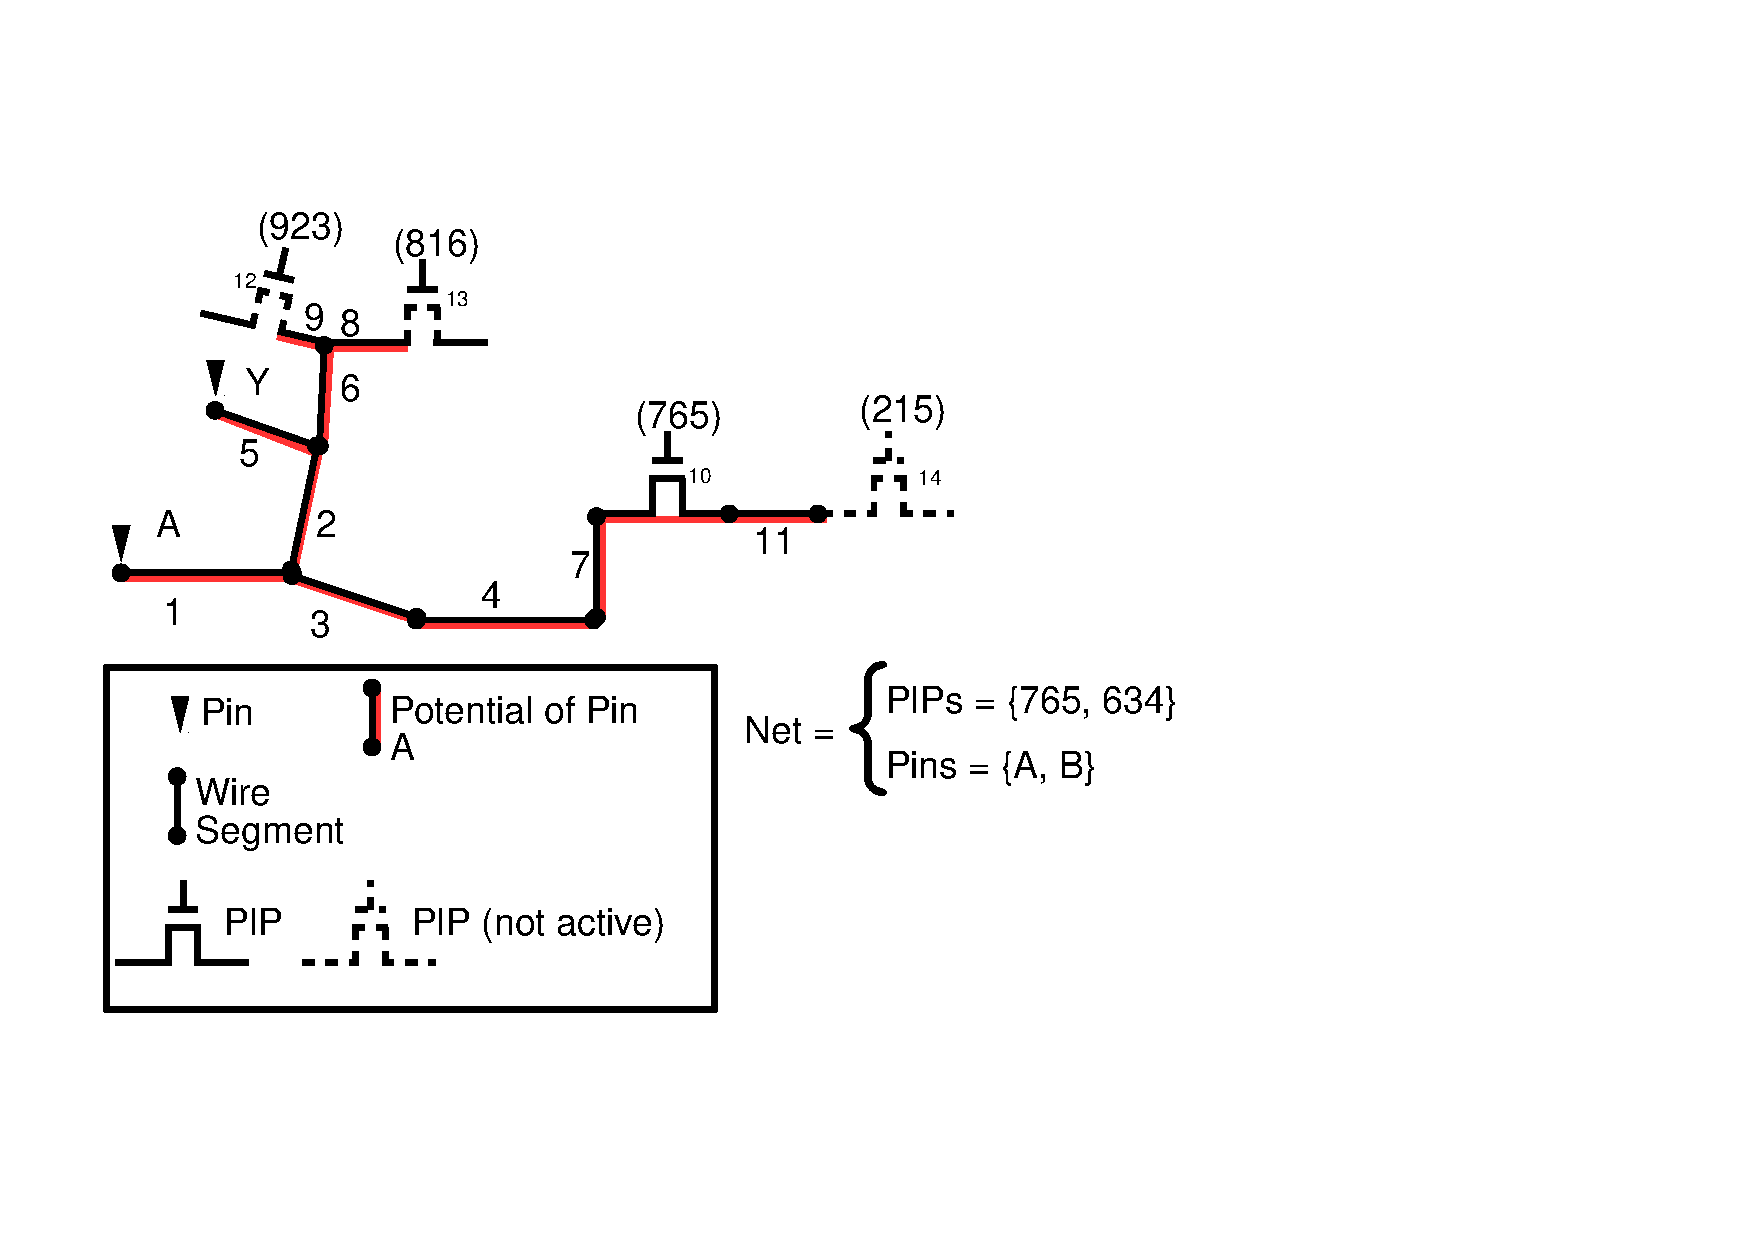
\includegraphics[scale=0.8]{images/buildpotential_buildup.pdf}
\caption{Graphical visualization of the \texttt{Potential} derivation. The wire segments and elements are enumerated in the sequence of integration. PIP IDs are in parentheses.}
\label{fig:buildpotential}
\end{figure}



\texttt{Potential}s can be fused by setting PIPs. Electrically, this means that two isoelectric sets of elements are connected by a switch, and thus become one isoelectric potential. For the object representation this means that, if a PIP is set, the two \texttt{Potential} objects have to be united.

The concept of isoelectric potentials is chosen because the search for adjacent pips wire by wire is simplified this way.



\section{Finding and Reparing broken Nets}
\label{sec:findingandrepairingbrokennets}

In order to check if an net is broken the potential of each pin is calculated and compared. If the net contains more than one unique potential then the net is broken.
In that case it is necessary to reconnect the two parts (potentials) of that net. If the assumption that only one or two PIPs are missing is true, this can be done by the applying the following breadth-first-search on the \texttt{Potential}s of pins A and B:

There is a priority queue with the name \textit{leaves} which holds only PIP-elements that do not connect to other potential besides B. 
Each of these elements has a parent PIP which introduced the PIP into the queue. \textit{leaves} is ordered by the number of parents between the PIP and Potential A in ascending order.

\begin{algorithm}[h]
	leaves.addAll(potenialA.getAdjacentPIPs());\\
	\While{leaves.size() > 0}{
		PIPElement pip = leaves.pop(); \\
		\If{potenialB.isPIPOfPotential(pip)}{
			return pip; // we can determine the connection trough the parent PIPs
		}
		\ForEach{PIP p in pip.getAdjacentPIPs}{
			If{p!=pip.parent}
				leaves.push(p); //if p is of an other potenial then B we can not add it 
		}
	}
 \caption{Exemplary algorithm to determine missing PIPs by breadth-first-search}
 \label{alg:breadth-first-search}
\end{algorithm}


While \textit{leaves} not empty do:
	Get first PIP of \textit{leaves}
	If PIP has Potential B then done
	Add all adjecenten PIPs to leaves

Figure \ref{fig:brokenpotentials} shows the case for one non-set PIP in a net. The net specifies two pins, A and B. For both pins, the \texttt{Potential} has been determined. Clearly marked are the included wires, PIPs and other pins. PIP 215 is adjacent to both potentials. The breadth-first-search finds PIP 215 to be adjacent to both pins' potentials, so this PIP has to be set (a \texttt{PIP} instance is created for the conencted \texttt{wires} and added to the net). For situations where more than one PIP has to be set, the breadth-first-search steps one level down the search tree and repeats the search on every leaf. By going one level deeper, the first PIP in the priority queue has to be set.

As one can see, the breadth-first search runtime highly depends on the number of missing PIPs in the net. For every missing PIP, the number of elements to search is multiplied by the amount of adjacent PIPs to the Potential.

\begin{figure}
\centering
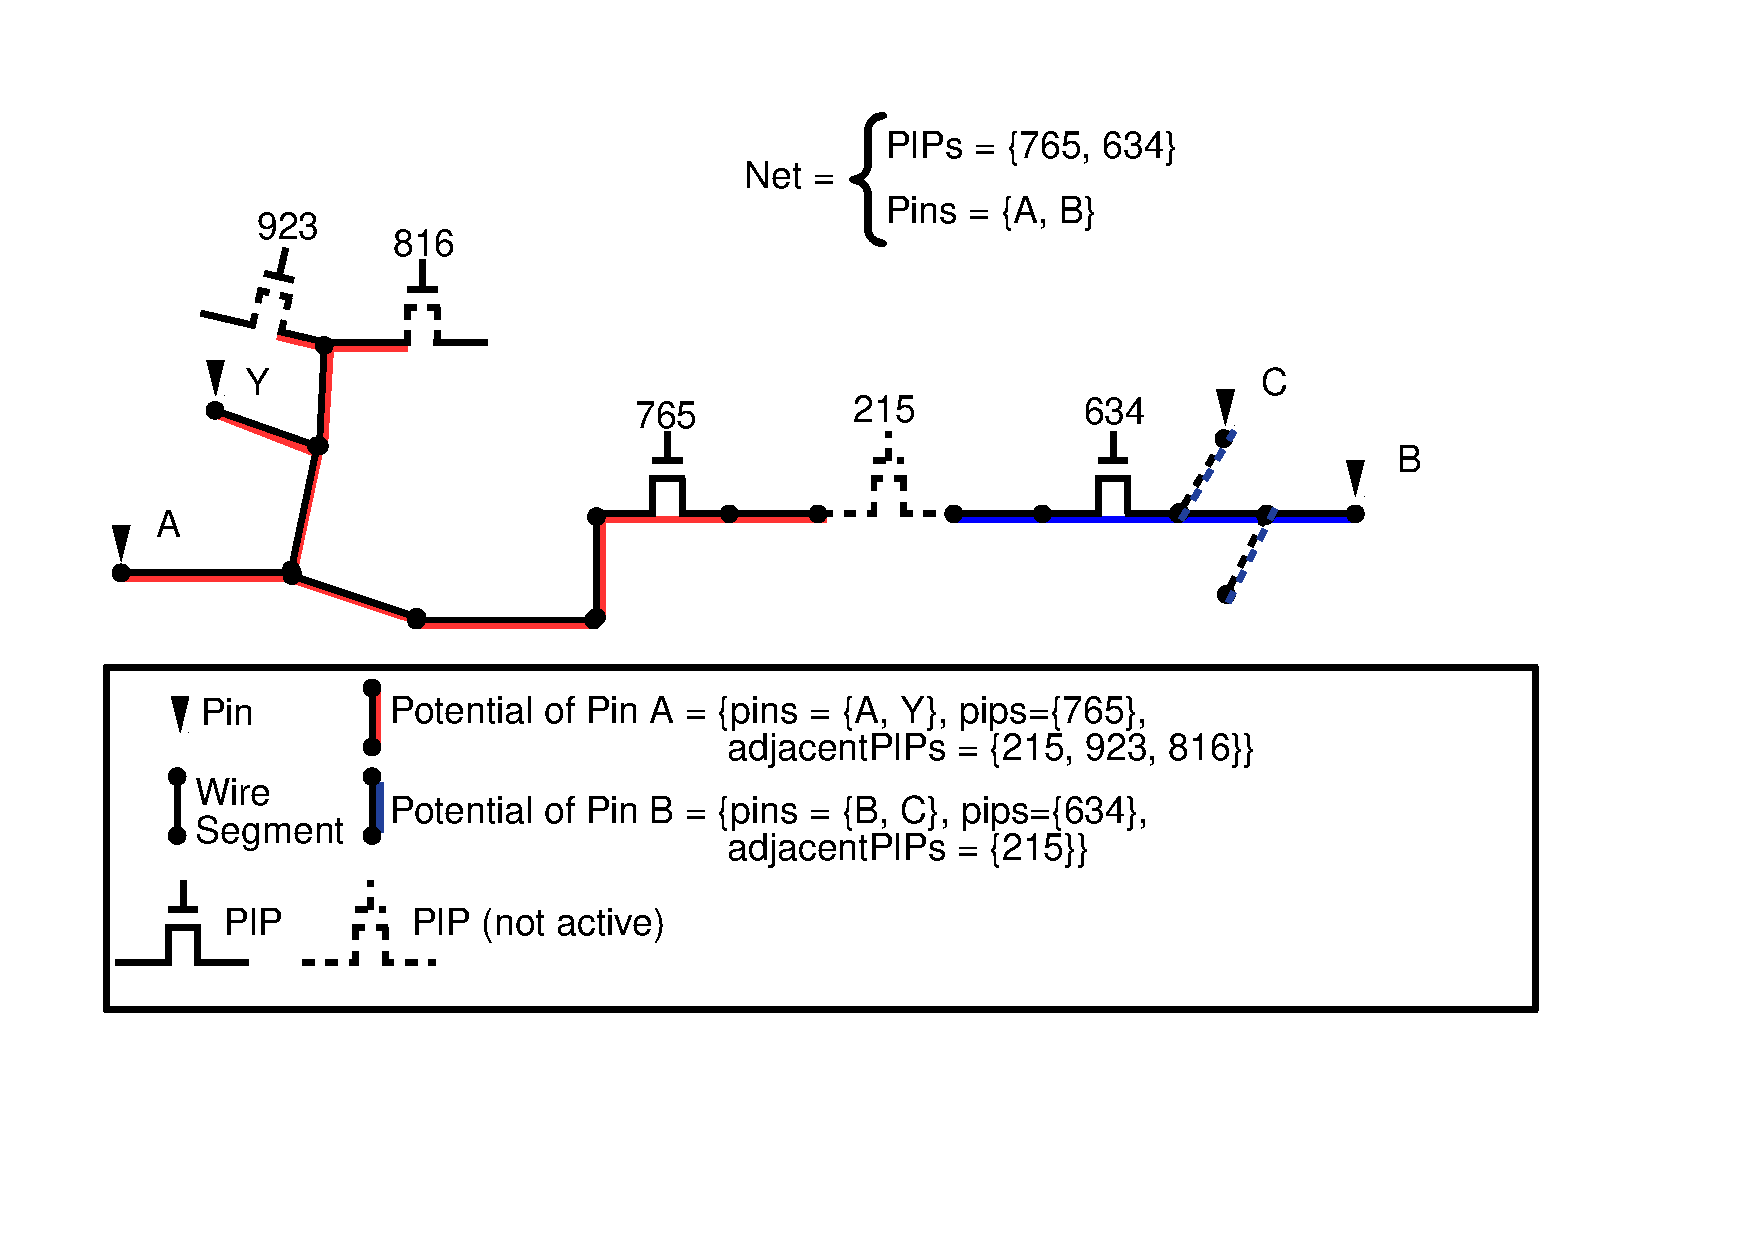
\includegraphics[scale=0.65]{images/brokenpotentials.pdf}
\caption{A net with two \texttt{Potentials} which have to be connected.}
\label{fig:brokenpotentials}
\end{figure}




% what we learned from the mini task
\chapter{Insights}
\label{cha:insights}

Although the approach described in chapter \ref{cha:approachestotheproblem} seems promising, testing it with diffrent designs and for various example nets (both conflicting and functional in terms of the ISE \texttt{xdl} output) did not lead to the expected results. Instead of finding exactly one potential per net most nets (more than 90\,\%) contains more than one potential. This behavior occurs regardless whether or not the design can be used by ISE and therefore has not to be rerouted.
Therefore, we examined the reasons, implementation and other possible error sources that may lead to this behavior.

\section{Hand Routing}
\label{sec:handrouting}

The RapidSmith framework has some built-in example classes, which are designed to help the user understand the way RapidSmith works. One of these classes is the \texttt{HandRouter}, which allows the routing of a net through a console. It displays reachable wires at the next iteration and adds PIPs as the route is chosen. We used and adapted the \texttt{HandRouter} to manually examine broken nets. Working on complete \texttt{.xdl}-files only, we adapted the router to work on single nets, and inserted it after the potential derivation.

Using the HandRouter reveals several error sources, but also that each connection reachable from each pin is correctly integrated in the pin's \texttt{Potential} instance. Therefore, we could prove that, based on the given nets, the concept of isoelectric potentials is implemented correctly. Nevertheless, the potentials of working designs were still not as expected.

Further analysis of the reacheable routing elements from every pin revealed that the assumption of only 1 or two missing PIPs between the isoelectric potentials of the sink and source pin evaluated to be wrong. In the most examined cases, at least four or more PIPs not specified by the net have to be additionally switched on. While some of the wire segments where additional PIPs are necessary only feature one or two switcheable PIPs, others had a much longer list. 

Therefore we were not able to determine which net is broken and therefore were not able to apply the breadth-first-search algorithm. In order to fix a design we would have to apply the algorithm on nearly every net of the design.  The breadth-first-search is suitable for search trees of one or two levels, in order to fulfill the purpose of this work, to save time during development, it is advisable to use a router able to solve the problem of many possible connections and a a larger number of PIPs.


%TODO: das gehört hier net hin
%Therefore, we decided not to apply the breadth-first-search and propose to perform a re-routing of the net. Any router has to solve the problem of too many possible connections on the route to take. The breadth-first-search is suitable for search trees of one or two levels, but it is probably bad compared to a distinct router able of finding routes with a larger number of PIPs.


\section{Possible Reasons for Errors}
\label{sec:possiblereasonsforerrors

The number of missing PIPs leads us to the assumption that the errors in re-placed designs or nets are not completely caused by small irregularities in the FPGA fabric. RapidSmith features a coordinate-based location description of nearly all elements of the FPGA. While this is useful for the majority of applications, some details may be hidden in this abstraction. Not every cartesian coordinate perfectly translates into the actual position of the element on the FPGA, so that regular structures in terms of the cartesian coordinates do not necessarily imply regular structures in the fabric. Hence, the assumption of conflicting re-placed nets caused by slight irregularities could not be proven.

In addition to the larger-than-expected irregularities, there are other error sources in RapidSmith. We cannot determine the exact source, but we have reason to assume that certain information on the FPGA are either missing or not correct. This assumption is made due to the fact even for functional nets (in terms of the \texttt{xdl} conversion), some of the corresponding RapidSmith \texttt{Net}s were not routed correctly (i.e. the source was reacheable from all sink pins).

\section{Outcome}
\label{sec:outcome}
Within this project, a method to find missing PIPs in re-placed FPGA designs was  developed. Its working principle is based on a breadth-first-search. According to the assumption that only very few PIPs are missing in the nets because of slight irregularities in the FPGA fabric, a breadth-first search is applicable. 

TODO DAS UNTEN GEHÖRT HIER NET HIN
Reviewing the results proves that there is either a problem with RapidSmith or the assumption of only few missing PIPs is wrong. In case that RapidSmith can be ruled out as an error source, we suggest the use of a dedicated router to repair the corrupted nets, because it is suited well for connecting elements with a higher amount of interconnect points between them. Of course, our approach to the problem is not the only possible; therefore, other solutions may produce better results.



% conclusion of this shit
\chapter{Conclusion}
\label{cha:conclusion}

The goal of this project was to determine and repair nets which are corrupted after a module re-placement due to slight irregularities in the FPGA fabric. This goal could partially be met. The analysis of corrupted nets is functional; although there is a method to fix the errors, we suggest a re-routing of the nets, because our solution is not applicable for the encountered error sources.

Our approach is based on isoelectric potentials, on which a breadth-first search finds missing interconnect elements. As pointed out in chapters \ref{cha:approachestotheproblem} and \ref{cha:insights}, the basic approach has correct results. Nevertheless, the errors encountered in the conflicting nets have shown to be of a kind which is not applicable to the breadth-first-search as solution. 

In conclusion it seems that there is currently no possibility to determine the exact properties of an net with RapidSmith based on the \texttt{.xdl} files. Corrupted nets can be found, but inconsistencies with the further processing complicate the possibility to distinguish between functional and corrupted nets.
During our experiments with the RapidSmith hand router we started to suspect that our database might be to small. Most nets, even those of not broken designs e.g. designs that can be used without a problem by the ISE tool-chain, contain no wires or other elements connecting the pins with each other. The few Nets that are connected are usually of a rather simplistic manner.
%Alternatively there is the possibility that RapidSmith might not be able
It should be noted that there is the slim possibility of bugs within RapidSmith. While we did not encounter any evidence for bugs we must note that the RapidSmith version used in this project showed some differences to the publicly available version on http://rapidsmith.sourceforge.net/. While most of these differences seem to be improvements, for example the wireEnumerator was upgraded by one version, it should also be noted that the GUI seems to be missing files.

All things considered, we recommend to use the algorithmic approach of this work with a bigger dataset or an alternative tool. For the meanwhile, we recommend to use a re-routing in case of error, because it is probably better than the suggested approach.

%
 % http://rapidsmith.sourceforge.net/papers/Nelson-FPL11-Presentation.pdf

%We suspect As shown in REF are X to Y big and ours are simply

%the task was to
%- examine re-placed designs' net lists

%- find out if something does not work

%- expected: only one or two PIPs are missing due to irreguar structure 
%of FPGA

%- if problem is encountered, find rule/mask based method to fix these 
%missing pips


%what we did was:

%- handle net by net 

%- for each Pin, determine all elements of the isoelectric it is 
%connected to (class potential)

%- checking method: if (potential(source)!=potential(sink) -> broken


%- for broken nets:

% - search isoelectric of source, sink for adjacent, non-set PIPs 
%(interesction of sets). if !=empty set, activate this pip


%- why it did not work:

%  - even for correct (in terms of make file) nets, the method fails

%  - hand routing (function of RapidSmith framework) neither does

%  - we suspect missing information in fabric;

%  - according to the hand router, the method of "isoelectric search" 

%results in correct sub nets; might be useful for later work



%% Anhang %%%%%%%%%%%%%%%%%%%%%%%%%%%%%%%%%%%%%%%%%%%%%%%%%%%%%%%%%%%%%%%%
%\appendix
\bibliographystyle{plain}
\clearpage
% \nocite{*}
\bibliography{literaturverzeichnis}


\end{document}
